\documentclass[11pt]{article}
\usepackage{arduino-uppgifter}

\newcommand{\mallurl}{https://wokwi.com/projects/357812594927244289}

% Figures subfolder
\graphicspath{{figures/}}

\begin{document}
\begin{center}
      \textbf{\huge{Introduktion till Arduino}}
      \huge{| MEKMEK01 v10}
\end{center}
\vspace{2em}

\begin{center}
      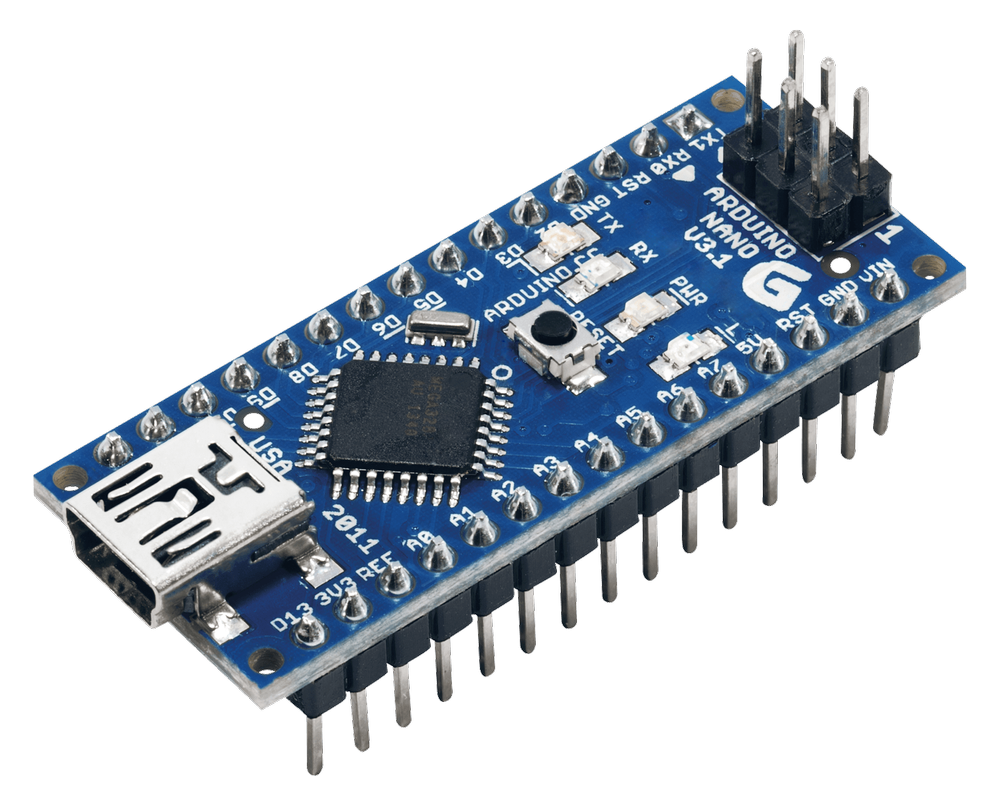
\includegraphics[width=0.4\textwidth]{nano}
\end{center}

\tableofcontents

\newpage
\raggedright{}
\section{Teori}
I uppgifterna kommer du lära känna Arduino genom praktiska övningar. Här kommer
lite kort teori om vad en Arduino är och vad den kan användas till.

\subsection{Vad är en mikrokontroller?}
En mikrokontroller är i princip en programmerbar liten dator som kan styra
elektronik. En mikrokontroller kan användas för att styra en mängd olika saker,
till exempel en robot, en lampa eller en kaffebryggare.
\begin{figure}[H]
      \centering
      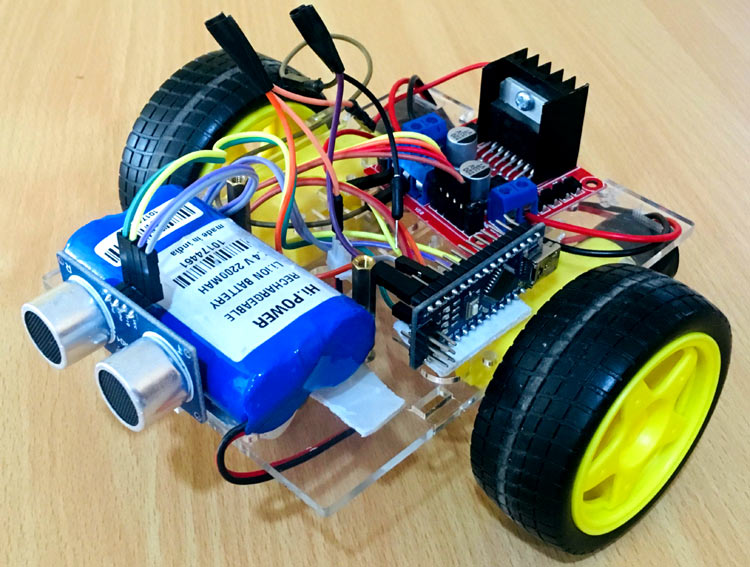
\includegraphics[width=0.5\textwidth]{obstacle_robot}
      \caption{En robot som använder en mikrokontroller för att undvika
            hinder.}
      \label{fig:obstacle_robot}
\end{figure}
\subsection{Vad är en Arduino?}
Arduino är som ett skal runt en mikrokontroller (vanligtvis AVR-processorer).
Den har en stor community som delar med sig av sina projekt och kod, så ni
kommer kunna använda det som inspiration för ert projekt. Det finns många olika
modeller av Arduino, men vi kommer använda oss av en \textbf{Arduino Nano}.

\subsection{Hur programmerar man en Arduino?}
Man skriver kod för Arduino i ett programmeringsspråk som liknar C++. Man kan
både skriva- och ladda upp koden till Arduino-enheten från en dator i
programmet \texttt{Arduino IDE}.

\newpage
\onehalfspacing
\section{Uppgifter}
Vi kommer att använda \texttt{Wokwi} för att simulera Arduino, både med
kretskopplingar och kod.
<<<<<<< HEAD
\subsection{Blink med \texttt{digitalWrite}}\label{sec:blink}
=======
\subsection{Blink med \texttt{digitalWrite} och \texttt{delay}}\label{sec:blink}
>>>>>>> c447678 (for next week)
Det enklaste programmet: blinka den interna lampan på Arduino-enheten med ett
fast intervall.

\begin{enumerate}[itemsep=1em]
      \item
            Öppna \href{\mallurl}{mallen för övningarna}
      \item
            Skriv in följande kod i \texttt{void setup()}:

            \begin{lstlisting}
pinMode(13, OUTPUT);
       \end{lstlisting}
      \item
            Skriv in följande kod i \texttt{void loop()}:

            \begin{lstlisting}
digitalWrite(13, HIGH);
delay(1000);
digitalWrite(13, LOW);
delay(1000);
       \end{lstlisting}
      \item
            Tryck på den gröna ``play''-knappen
            
\includegraphics[width=2em,valign=c]{play} för att starta
            simuleringen.
\end{enumerate}
\vspace{1em}
Vad ser du? Vad tror du att koden gör?

Vad händer om du ändrar \texttt{delay(1000)} till \texttt{delay(500)}?

Vad händer om du ändrar alla \texttt{13} till någon annan siffra? Vad betyder
siffran?

\newpage
\subsection{Knapp med \texttt{digitalRead}}\label{sec:knapp}
\begin{enumerate}
      \item
            Öppna \href{\mallurl}{mallen för övningarna}
      \item
            Skriv in följande kod i \texttt{void setup()}:
            \begin{lstlisting}
pinMode(2, INPUT);
pinMode(13, OUTPUT);
            \end{lstlisting}
      \item
            Skriv in följande kod i \texttt{void loop()}:
            \begin{lstlisting}
bool buttonValue = digitalRead(2);
digitalWrite(13, buttonValue);
                  \end{lstlisting}
      \item
            Lägg till en knapp i kretsen genom att klicka plus-knappen
            
\includegraphics[width=2em,valign=c]{plus} och sedan välja
            ``Pushbutton''. Lägg till en resistor på 10 k$\Omega$ på samma
            sätt.
      \item
            Koppla ihop allting enligt figur \ref{fig:knapp_setup} nedan. Du
            drar sladdar genom att klicka på en kopplingspunkt och sedan på en
            annan
            kopplingspunkt.
            \begin{figure}[H]
                  \centering
                  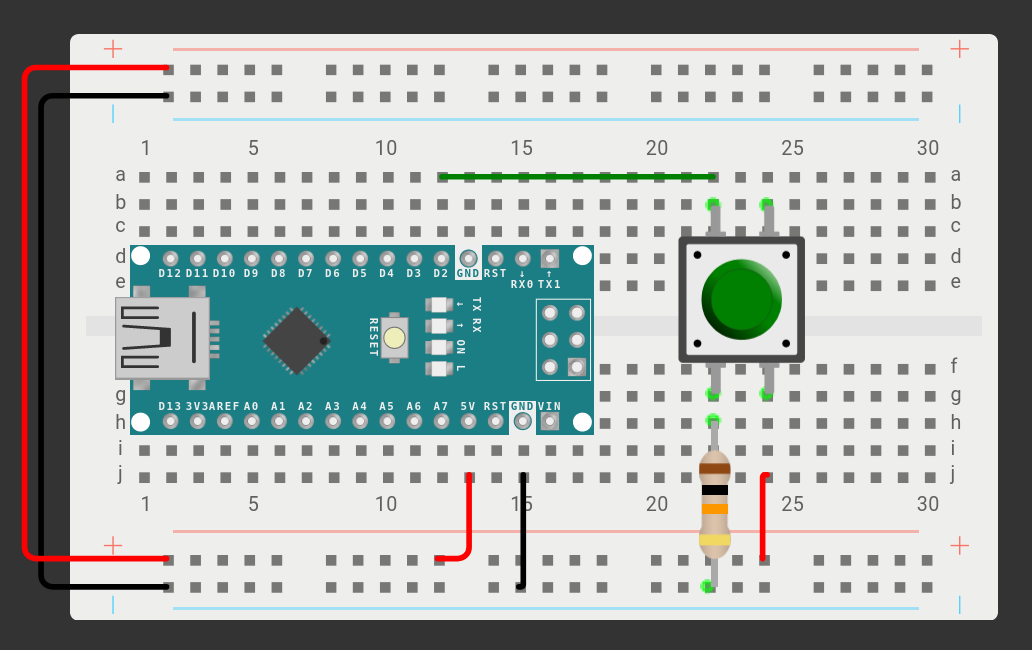
\includegraphics[width=.8\textwidth]{knapp_setup}
                  \caption{Krets med knapp och resistor}
                  \label{fig:knapp_setup}
            \end{figure}
      \item
            Starta simuleringen som i förra uppgiften \nameref{sec:blink}.
      \item
            Testa att trycka på knappen med musmarkören. Vad händer?
      \item
            Testa att ta bort resistorn. Vad händer? Vad är resistorns syfte?
\end{enumerate}

\newpage
\subsection{Seriell kommunikation med \texttt{Serial}}\label{sec:serial}
Arduinon kan ``print:a'' precis som du är van vid i andra programmeringsspråk.
För att göra detta måste den vara ansluten till en dator via USB. Detta kan
vara
användbart när man felsöker eller vill skicka data till datorn. Vi ska nu
skriva ett program som räknar antal gånger en knapp trycks på och skickar detta
till datorn.

\begin{enumerate}[itemsep=1em]
      \item
            Fortsätt från \nameref{sec:knapp}
      \item Skriv in följande kod högst upp i filen, utanför funktionerna:
            \begin{lstlisting}
int count = 0;
            \end{lstlisting}
      \item Skriv in följande kod i \texttt{void setup()}:
            \begin{lstlisting}
pinMode(2, INPUT);
Serial.begin(9600);
            \end{lstlisting}
      \item Skriv in följande kod i \texttt{void loop()}:
            \begin{lstlisting}
bool buttonValue = digitalRead(2);
if (buttonValue) {
  count++;
  Serial.println(count);
}
            \end{lstlisting}
      \item Starta simuleringen. Nu öppnas en terminal längst ner i skärmen.
      \item Tryck på knappen och se vad som händer i terminalen.
\end{enumerate}
\vspace{1em}
Varför tror du att vi skriver \texttt{Serial.begin(9600);} i \texttt{void
      setup()}?

Vad betyder \texttt{Serial.println(count);}? Vad händer om du ändrar det till
\texttt{Serial.print(count);}?

\newpage
\subsection{Reaktionstest med \texttt{millis}}
Nu ska vi skapa ett lite mer avancerat program- ett reaktionstest.
Arduinons inbyggda funktion
\texttt{\href{https://www.arduino.cc/reference/en/language/functions/time/millis/}{millis()}}
kan användas för att mäta hur långt tid som har passerat sedan den startats.

\begin{enumerate}[itemsep=1em]
      \item
            Fortsätt från \nameref{sec:knapp}
      \item Skriv in följande kod i \texttt{void setup()}:
            \begin{lstlisting}
pinMode(BTN_PIN, INPUT);
pinMode(13, OUTPUT);
            \end{lstlisting}
      \item Skriv in följande kod i \texttt{void loop()}:
            \begin{lstlisting}
digitalWrite(13, HIGH);

while (digitalRead(BTN_PIN) == LOW) {} // Vänta tills knapp trycks

digitalWrite(13, LOW);
Serial.println("Tryck så fort du ser lampan lysa!");

delay(random(1000,5000)); // Vänta slumpmässigt mellan 1-5 sekunder

digitalWrite(13, HIGH);
Serial.println("Nu!!");

int millisBefore = millis();
while (digitalRead(BTN_PIN) == LOW) {} // Vänta tills knapp trycks

digitalWrite(13, LOW);
int reactionTime = millis() - millisBefore; // Räkna ut reaktionstid
Serial.print("Din reaktionstid: ");
Serial.print(reactionTime);
Serial.println("millisekunder");

delay(1000); // Vänta tills man kan börja reaktionstestet igen
                  \end{lstlisting}
      \item Försök att starta simuleringen. Varför funkar det inte?

            \textbf{Tips: } Läs vad kompilatorn ``klagar'' på. Kan du fixa det?
      \item När du har fått igång simuleringen, testa programmet genom att
            trycka på knappen. Ser du någonting i \texttt{Serial Monitor}
            (terminalen i
            nedre delen av skärmen)? Varför inte?

            \textbf{Tips: } Läs igenom koden från
            \nameref{sec:serial}.
\end{enumerate}


\end{document}